\documentclass[11pt]{article}
\usepackage[margin=2.5cm]{geometry}
\usepackage[utf8]{inputenc}
\usepackage[T1]{fontenc}
\usepackage{graphicx}
\usepackage{booktabs}
\usepackage{longtable}
\usepackage{xcolor}
\usepackage{hyperref}
\usepackage{siunitx}
\usepackage{caption}
\hypersetup{colorlinks=false, pdfborder={0 0 0}}

\definecolor{okgreen}{RGB}{0,120,60}
\definecolor{warnred}{RGB}{180,30,30}
\definecolor{sugamber}{RGB}{170,110,0}

\title{ComplexCalc-HW --- Power Supply Review}
\author{}
\date{}

\begin{document}
\maketitle
\vspace{-1.3cm}

\section{Purpose}

This document summarizes the official power supply requirements of the
STM32F411CEUx (datasheet DocID026289 Rev.\,7, ST\-Microelectronics) for the
\textbf{UFQFPN48} package, and compares them against what is currently
routed in \texttt{design/\allowbreak ComplexCalc/\allowbreak
ComplexCalc.kicad\_sch} of the \texttt{UAA-F14/\allowbreak ComplexCalc-HW}
repository. All reference figures and tables are direct captures from the
official datasheet.

\section{Actual pinout: UFQFPN48}

Figure~\ref{fig:pinout} (Figure~10 of the datasheet, page~34) shows the
exact pin assignment of the package used on this board. From it we
confirm:

\begin{itemize}
  \item \textbf{3 VDD pins}: 24, 36, 48
  \item \textbf{3 VSS pins}: 23, 35, 47
  \item \textbf{Only 1 VCAP\_1 pin} (pin 22) --- this package does
        \emph{not} bring out VCAP\_2 (that signal only exists on the
        LQFP100 and UFBGA100 packages)
  \item VBAT: pin 1
  \item VDDA/VREF+: pin 9 · VSSA/VREF-: pin 8
  \item NRST: pin 7 · BOOT0: pin 44
\end{itemize}

\begin{figure}[h]
  \centering
  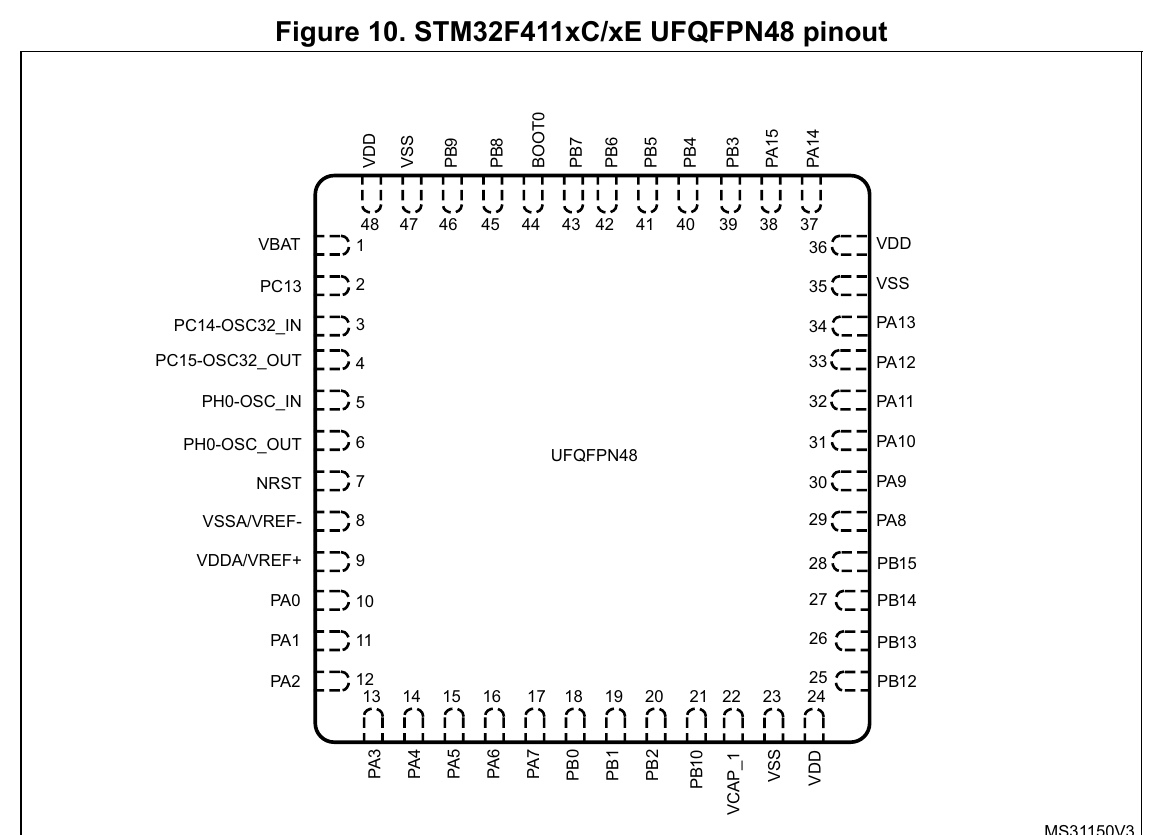
\includegraphics[width=0.58\textwidth]{figs/pinout-034-crop.png}
  \caption{UFQFPN48 pinout --- Figure 10, STM32F411xC/xE datasheet, p.~34}
  \label{fig:pinout}
\end{figure}

\clearpage
\section{Official power supply scheme}

Figure~\ref{fig:powerscheme} (Figure~17, Section 6.1.6, page~59) is ST's
reference scheme for decoupling each power supply branch.

\begin{figure}[h]
  \centering
  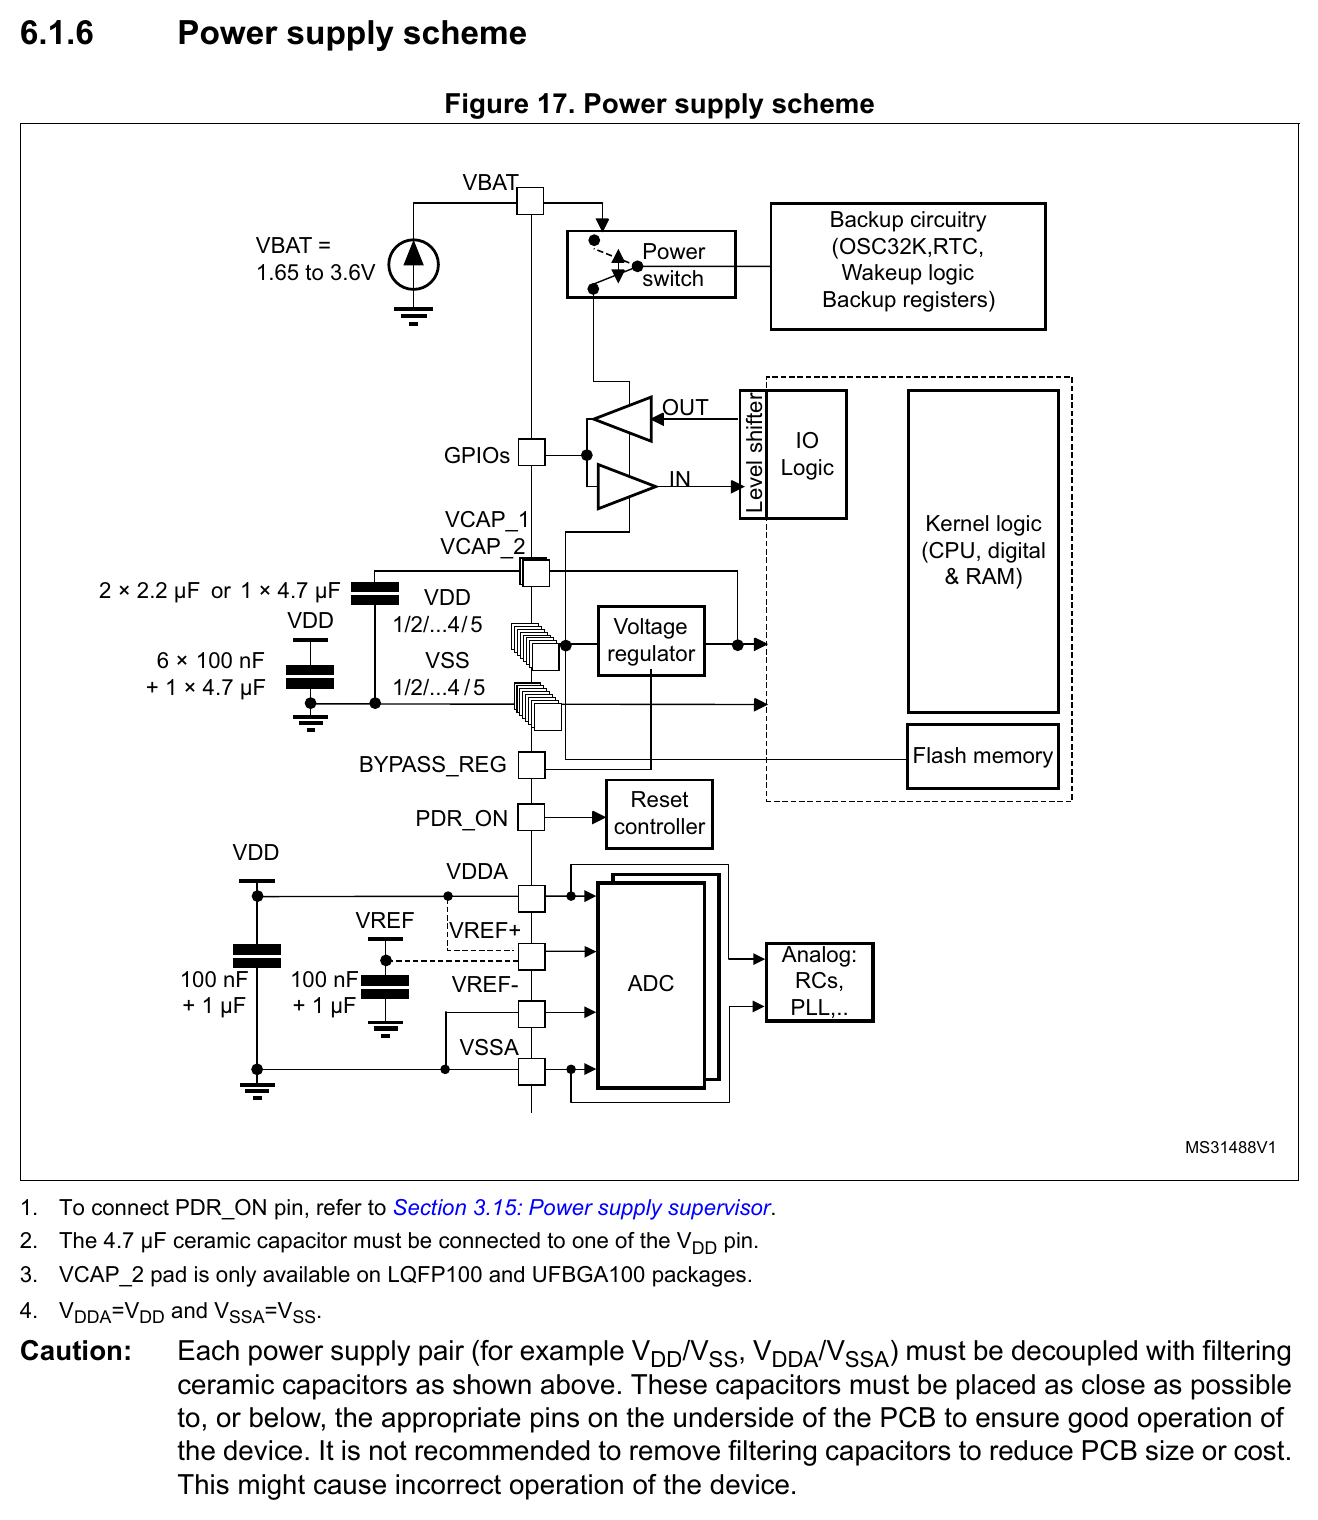
\includegraphics[width=0.72\textwidth,height=0.78\textheight,keepaspectratio]{figs/powerscheme-059-crop.png}
  \caption{Power supply scheme --- Figure 17, Section 6.1.6, p.~59}
  \label{fig:powerscheme}
\end{figure}

\newpage
\section{VCAP capacitor for single-pin packages}

Table~\ref{fig:vcaptable} (Table~16, Section 6.3.2, page~65) gives the
exact value that applies specifically when the package brings out only one
VCAP pin (our case).

\begin{figure}[h]
  \centering
  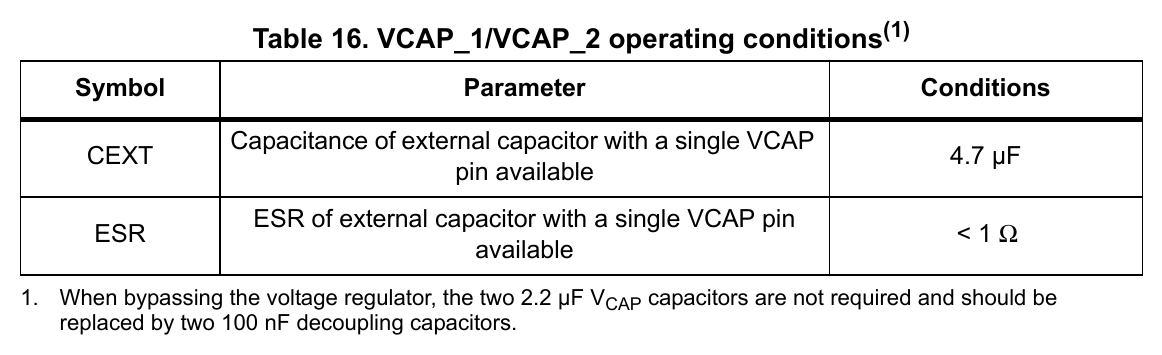
\includegraphics[width=0.8\textwidth]{figs/vcaptable-065-crop.png}
  \caption{VCAP\_1/VCAP\_2 operating conditions --- Table 16, Section 6.3.2, p.~65}
  \label{fig:vcaptable}
\end{figure}

\section{Summary: required values per pin}

\begin{longtable}{p{3.2cm}p{4.5cm}p{6cm}}
\toprule
\textbf{Pin(s)} & \textbf{Required capacitor(s)} & \textbf{Source} \\
\midrule
\endhead
VDD / VSS (pins 24/23, 36/35, 48/47) &
  100\,nF per VDD/VSS pair (3 total) + 1$\times$4.7\,µF on any of the
  VDD pins &
  Figure~17, note~2 \\
VCAP\_1 (pin 22) $\rightarrow$ GND &
  \textbf{4.7\,µF ceramic, ESR $<$ 1\,$\Omega$} (single-VCAP package) &
  Table~16, Section~6.3.2 \\
VDDA/VREF+ (pin 9) $\leftrightarrow$ VSSA/VREF- (pin 8) &
  100\,nF + 1\,µF (single pair: on this package VDDA and VREF+ share a
  pin) &
  Figure~17 \\
VBAT (pin 1) &
  100\,nF, or a direct connection to VDD if no backup battery is used &
  Figure~17 \\
NRST (pin 7) &
  Already has an internal pull-up --- an external capacitor (100\,nF,
  optional) only improves EMI immunity, it is not mandatory &
  Table~7 (NRST legend) \\
BOOT0 (pin 44) &
  No internal bias --- external resistor (typ. 10\,k$\Omega$ pull-down
  to boot from flash) &
  Section 3.13 ``Boot modes'' \\
\bottomrule
\end{longtable}

\clearpage
\section{Comparison against the actual schematic}

Extracted from the \texttt{ComplexCalc.kicad\_sch} netlist (exported with
\texttt{kicad-cli}) on September 2, 2026.

\begin{longtable}{p{3.5cm}p{3.2cm}p{3.2cm}p{4cm}}
\toprule
\textbf{Checked item} & \textbf{Required} & \textbf{In the schematic} & \textbf{Verdict} \\
\midrule
\endhead
VCAP\_1 (C14) & 4.7\,µF, ESR$<$1$\Omega$ & \textbf{2.2\,µF} &
  \textcolor{warnred}{\textbf{Below the required value}} --- 2.2\,µF is
  the value for packages with \emph{two} VCAP pins, not a single one. \\
VBAT (pin 1) & Tied to battery or to VDD & \textbf{Unconnected (isolated
  net)} & \textcolor{warnred}{\textbf{Floating}} --- it is neither on the
  3.3\,V net nor does it have a capacitor. \\
VDD/VSS (3 pairs) & 3$\times$100\,nF + 1 bulk & C10, C11, C12 (100\,nF
  each) + C13 (1\,µF) + C8 (22\,µF) &
  \textcolor{okgreen}{Meets the requirement} --- bulk capacitance is even
  larger than the minimum required. \\
VDDA/VREF+ (pin 9) & 100\,nF + 1\,µF local & Same 3.3\,V net as VDD, with
  C13 (1\,µF) present & \textcolor{okgreen}{Electrically compliant} ---
  physical proximity of the capacitor to the pin could not be verified
  from the schematic (check the layout). \\
NRST & Internal pull-up already sufficient; typ.\ cap.\ 100\,nF & R4
  (10\,k$\Omega$ external, redundant) + C9 (\textbf{1\,µF}, not 100\,nF) &
  \textcolor{sugamber}{\textbf{Suggest lowering to 100\,nF}} --- not an
  error (it is still functional), but 1\,µF extends the reset time more
  than necessary. Confirmed against the actual BlackPill schematic (WeAct
  Studio): its reset circuit uses exactly \textbf{100\,nF} at the same
  node. \\
BOOT0 (R5) & $\sim$10\,k$\Omega$ pull-down & 10\,k$\Omega$ &
  \textcolor{okgreen}{Correct} \\
BOOT1/PB2 (R6) & Define level & 10\,k$\Omega$ pull &
  \textcolor{okgreen}{Correct} \\
HSE crystal (Y1) & Must match \texttt{RCC.HSE\_VALUE} in firmware &
  Y1 = \textbf{8\,MHz} physically, but the \texttt{.ioc} has
  \texttt{HSE\_VALUE=25000000} & \textcolor{warnred}{\textbf{Review}} ---
  if the firmware ever enables HSE, the clock tree must be recalculated
  for 8\,MHz, not 25\,MHz. \\
Regulator (U2) & --- & \textbf{AMS1117-3.3} (not NCP1117-3.3) &
  Documentation note: corrected in the repo's README. \\
\bottomrule
\end{longtable}

\section{Recommended actions}

\begin{enumerate}
  \item Change C14 from 2.2\,µF to \textbf{4.7\,µF} on VCAP\_1.
  \item Connect VBAT (pin 1) to the 3.3\,V rail (or leave a 100\,nF
        footprint if a real backup battery for the RTC is added in the
        future).
  \item Lower C9 (NRST) from 1\,µF to \textbf{100\,nF} --- the textbook
        value, and the one used by the actual reference BlackPill at the
        same node.
  \item Before enabling HSE in firmware, correct \texttt{RCC.HSE\_VALUE}
        to 8\,MHz in the \texttt{.ioc} and regenerate the clock tree in
        STM32CubeMX.
  \item Verify on the physical layout (not just the schematic) that the
        VDD/VDDA capacitors are placed as close as possible to their
        respective pins, since the bottom layer is already occupied by
        the matrix keypad.
\end{enumerate}

\end{document}
